\lecture{9}{Machine Learning with Heterogeneous Graphs}{Tuesday, October 20, 2026}\label{ch:lec09}

\providecommand{\mV}{\mathbf{V}}

% Local TikZ styles (prefix lec09)
\tikzset{
  lec09A/.style={fill=Goldenrod!70},
  lec09B/.style={fill=BrickRed!60},
  lec09C/.style={fill=ForestGreen!50},
  lec09D/.style={fill=RoyalBlue!45},
  lec09E/.style={fill=Orchid!60},
  lec09F/.style={fill=WildStrawberry!45},
  lec09n/.style={circle, draw=black!60, thick, minimum size=4.6mm,
                 inner sep=0pt, font=\scriptsize\sffamily},
  lec09r1/.style={thick, Cerulean, -{Stealth[length=1.8mm]}},
  lec09r2/.style={thick, BrickRed!85, -{Stealth[length=1.8mm]}},
  lec09r3/.style={thick, Goldenrod!90!black, -{Stealth[length=1.8mm]}},
  lec09lbl/.style={font=\scriptsize, inner sep=1.5pt},
  lec09agg/.style={draw=black!60, thick, fill=black!12, minimum size=5mm},
  lec09w/.style={draw=black!60, minimum width=1.7mm, minimum height=5mm,
                 inner sep=0pt},
  lec09ar/.style={black!75, -{Stealth[length=1.5mm]}},
  lec09paper/.style={circle, draw=black!80, thick, fill=BrickRed!60,
                     minimum size=3.8mm, inner sep=0pt},
  lec09author/.style={circle, draw=black!80, thick, fill=RoyalBlue!60,
                      minimum size=3.8mm, inner sep=0pt},
  lec09like/.style={line width=1.5pt, Goldenrod!85!black},
  lec09cite/.style={line width=1.5pt, ForestGreen!75},
  lec09v/.style={circle, draw=black!55, thick, minimum size=13mm,
                 align=center, font=\scriptsize\sffamily, inner sep=0.5pt},
  lec09lin/.style={draw, thick, fill=white, font=\scriptsize,
                   minimum height=5.5mm, inner sep=2.5pt},
}

\textbf{Outline.} So far: graphs with one edge type $\to$ graphs with multiple
node or edge types (a.k.a.\ \term{heterogeneous graphs}). Goal: learning with
heterogeneous graphs: Relational GCNs $\to$ design space for heterogeneous GNNs
$\to$ Heterogeneous Graph Transformer (time permitting).

% ---------------------------------------------------------------------
\section{Heterogeneous graphs}\label{sec:lec09-hetero}

\subsection{Motivation and definition}\label{sec:lec09-def}
\slides{3--9}

\begin{itemize}
  \item \textbf{2 types of nodes:} node type A: \textbf{paper} nodes; node type
    B: \textbf{author} nodes. \textbf{2 types of edges:} edge type A:
    \textbf{Like}; edge type B: \textbf{Cite} (\cref{fig:lec09-toy}).
  \item A graph could have multiple types of nodes and edges! \textbf{2 types of
    nodes + 2 types of edges} $\Rightarrow$ \textbf{8 possible relation types!}
  \item \term{Relation types}: (node\_start, edge, node\_end).
    \begin{itemize}
      \item We use \textbf{relation type to describe an edge} (as opposed to
        edge type).
      \item Relation type better captures the interaction between nodes and
        edges.
    \end{itemize}
\end{itemize}

\begin{figure}[htbp]
  \centering
  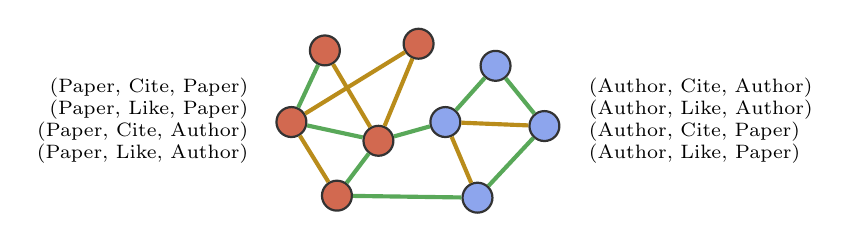
\begin{tikzpicture}[scale=0.85]
    \node[lec09paper] (p1) at (-1.4,1.05) {};
    \node[lec09paper] (p2) at (0.0,1.15) {};
    \node[lec09paper] (p3) at (-1.9,-0.02) {};
    \node[lec09paper] (p4) at (-0.6,-0.3) {};
    \node[lec09paper] (p5) at (-1.22,-1.12) {};
    \node[lec09author] (a1) at (1.15,0.82) {};
    \node[lec09author] (a2) at (0.4,-0.02) {};
    \node[lec09author] (a3) at (1.88,-0.08) {};
    \node[lec09author] (a4) at (0.88,-1.15) {};
    \draw[lec09cite] (p1) -- (p3);  \draw[lec09like] (p1) -- (p4);
    \draw[lec09like] (p3) -- (p2);  \draw[lec09like] (p2) -- (p4);
    \draw[lec09cite] (p3) -- (p4);  \draw[lec09like] (p3) -- (p5);
    \draw[lec09cite] (p5) -- (p4);  \draw[lec09cite] (p4) -- (a2);
    \draw[lec09cite] (a2) -- (a1);  \draw[lec09cite] (a1) -- (a3);
    \draw[lec09like] (a2) -- (a3);  \draw[lec09like] (a2) -- (a4);
    \draw[lec09cite] (a4) -- (a3);  \draw[lec09cite] (p5) -- (a4);
    \node[align=right, anchor=east, font=\scriptsize] at (-2.4,0)
      {(Paper, Cite, Paper)\\(Paper, Like, Paper)\\(Paper, Cite, Author)\\(Paper, Like, Author)};
    \node[align=left, anchor=west, font=\scriptsize] at (2.4,0)
      {(Author, Cite, Author)\\(Author, Like, Author)\\(Author, Cite, Paper)\\(Author, Like, Paper)};
  \end{tikzpicture}
  \caption{2 node types (red: paper, blue: author) + 2 edge types (gold: Like,
  green: Cite) and the 8 possible relation types (slides~5--8).}
  \label{fig:lec09-toy}
\end{figure}

\begin{definition}[Heterogeneous graph]\label{def:lec09-hetero}
  A heterogeneous graph is defined as
  \begin{equation}\label{eq:lec09-hetero}
    \bm{G} = (\bm{V}, \bm{E}, \tau, \phi)
  \end{equation}
  \begin{itemize}
    \item \textbf{Nodes with node types} $v\in V$; \textbf{node type} for node
      $v$: $\tau(v)$.
    \item \textbf{Edges with edge types} $(u,v)\in E$ (an edge can be described
      as a pair of nodes); \textbf{edge type} for edge $(u,v)$: $\phi(u,v)$.
    \item \textbf{Relation type} for edge $e$ is a tuple:
      $r(u,v) = \big(\tau(u), \phi(u,v), \tau(v)\big)$.
  \end{itemize}
\end{definition}
\begin{itemize}
  \item There are other definitions for heterogeneous graphs as well -- they
    describe \textbf{graphs with node \& edge types}.
\end{itemize}

\subsection{Many graphs are heterogeneous graphs}\label{sec:lec09-examples}
\slides{10--12}

\begin{itemize}
  \item \textbf{Biomedical knowledge graphs} (node types in figure: drug,
    disease, adverse event, protein, pathways; edges e.g.\ TREATS, CAUSES,
    ASSOC, IS\_A, HAS\_FUNC). Example node: \textbf{Migraine}; example relation:
    \textbf{(fulvestrant, Treats, Breast Neoplasms)}; example node type:
    \textbf{Protein}; example edge type: \textbf{Causes}.
  \item \textbf{Event graphs} (node types in figure: flight, airport, cause;
    edges: origin, destination, cancelled by, delayed by, diverted to). Example
    node: \textbf{SFO}; example relation: \textbf{(UA689, Origin, LAX)}; example
    node type: \textbf{Flight}; example edge type: \textbf{Destination}.
  \item \textbf{E-commerce graph}: node types User, Item, Query, Location,
    \dots; edge types Purchase, Visit, Guide, Search, \dots\ (figure: users
    Search queries ``Shoes'', ``Ladies Bag'' and Click items; Guide links items
    to queries ``Shoes'', ``Ladies Bag'', ``Hand Bag''). \textbf{Different node
    type's feature spaces can be different!}
  \item \textbf{Academic graph}: node types Author, Paper, Venue, Field, \dots;
    edge types Publish, Cite, \dots\ (figure: authors publish in KDD / ICML /
    AAAI; venues belong to fields Mining / Vision / Machine Learning; venues
    cite venues). Benchmark dataset: \textbf{Microsoft Academic Graph}.
\end{itemize}

\subsection{Discussion: type or feature?}\label{sec:lec09-typefeat}
\slides{13--15}

\begin{itemize}
  \item \textbf{Observation:} we can also treat types of nodes and edges as
    features.
    \begin{itemize}
      \item \textbf{Example:} add a one-hot indicator for nodes and edges: append
        feature $[1,0]$ to each ``author node''; append feature $[0,1]$ to each
        ``paper node''; similarly, assign edge features to edges with different
        types.
      \item Then, a heterogeneous graph \textbf{reduces to a standard graph}.
    \end{itemize}
  \item \textbf{When do we need a heterogeneous graph?}
    \begin{itemize}
      \item \textbf{Case 1:} different node/edge types \textbf{have different
        shapes of features}: an ``author node'' has 4-dim feature, a ``paper
        node'' has 5-dim feature.
      \item \textbf{Case 2:} we know different relation types represent
        \textbf{different types of interactions}: (English, translate, French)
        and (English, translate, Chinese) require different models.
    \end{itemize}
  \item There are many ways to \textbf{convert a heterogeneous graph to a
    standard graph} (that is, a homogeneous graph).
\end{itemize}
\begin{keyidea}
  Ultimately, a \textbf{heterogeneous graph is a more expressive graph
  representation}: it captures \textbf{different types of interactions between
  entities}. But it also \textbf{comes with costs}: more expensive (computation,
  storage); more complex implementation.
\end{keyidea}

% ---------------------------------------------------------------------
\section{Relational GCN (RGCN)}\label{sec:lec09-rgcn}

\subsection{From GCN to RGCN}\label{sec:lec09-gcn2rgcn}
\slides{16--24}

\begin{itemize}
  \item \textbf{Recap: GCN} (Kipf \& Welling, ICLR 2017; \cref{ch:lec04}):
    $\vh_v^{(l)} = \sigma\big(\mW^{(l)}\sum_{u\in N(v)}\frac{\vh_u^{(l-1)}}{|N(v)|}\big)
    = \sigma\big(\sum_{u\in N(v)}\mW^{(l)}\frac{\vh_u^{(l-1)}}{|N(v)|}\big)$:
    message $\mW^{(l)}\frac{\vh_u^{(l-1)}}{|N(v)|}$, aggregation
    $\sum_{u\in N(v)}$.
  \item \textbf{We will extend GCN to handle heterogeneous graphs with multiple
    edge/relation types.}
  \item We start with a \textbf{directed graph} with \textbf{one} relation: how do
    we run GCN and update the representation of the \textbf{target node $A$}?
    $\Rightarrow$ \textbf{Only pass messages along direction of edges}
    (computation graph: $A\leftarrow\{B,C,D\}$, $B\leftarrow C$,
    $C\leftarrow\{F,E\}$).
  \item What if the graph has \textbf{multiple relation types} ($r_1,r_2,r_3$,
    \cref{fig:lec09-rgcn})? $\Rightarrow$ \textbf{use different neural network
    weights for different relation types}: weights $\mW_{r_1}$ for $r_1$,
    $\mW_{r_2}$ for $r_2$, $\mW_{r_3}$ for $r_3$. In the computation graph, each
    message passes through the neural network of its relation, then aggregation.
  \item \textbf{Recap GCN + we add a self-loop:}
\end{itemize}
\begin{equation}\label{eq:lec09-gcn-self}
  \vh_v^{(l)} = \sigma\Big(\sum_{u\in N(v)}\mW^{(l)}\frac{\vh_u^{(l-1)}}{|N(v)|}
    + \mW^{(l)}\vh_v^{(l-1)}\Big)
\end{equation}
\begin{itemize}
  \item \textbf{Introduce a set of neural networks for each relation type!}
    Weight for rel\_1, \dots, weight for rel\_N, \textbf{weight for self-loop}
    (figure: each relation rel\_1, \dots, rel\_N forms its own graph around the
    node).
\end{itemize}

\begin{figure}[htbp]
  \centering
  \begin{tikzpicture}[scale=0.85]
    % input graph
    \node[lec09n, lec09A] (A) at (0,0) {A};
    \node[lec09n, lec09B] (B) at (1.5,0.6) {B};
    \node[lec09n, lec09C] (C) at (1.8,-0.25) {C};
    \node[lec09n, lec09D] (D) at (-0.8,-1.2) {D};
    \node[lec09n, lec09E] (E) at (0.95,-1.2) {E};
    \node[lec09n, lec09F] (F) at (2.45,-1.0) {F};
    \draw[lec09r1] (B) -- node[above left, lec09lbl, Cerulean] {$r_1$} (A);
    \draw[lec09r1] (D) -- node[left, lec09lbl, Cerulean] {$r_1$} (A);
    \draw[lec09r2] (C) -- node[below, lec09lbl, BrickRed] {$r_2$} (A);
    \draw[lec09r3] (C) -- node[right, lec09lbl, Goldenrod!90!black] {$r_3$} (B);
    \draw[lec09r3] (E) -- node[left, lec09lbl, Goldenrod!90!black] {$r_3$} (C);
    \draw[lec09r2] (F) -- node[pos=0.6, right, lec09lbl, BrickRed] {$r_2$} (C);
    \draw[lec09r1] (F) -- node[below, lec09lbl, Cerulean] {$r_1$} (E);
    \node[font=\scriptsize\sffamily, left=2pt of A] {target node};
    \node[font=\scriptsize\sffamily] at (0.8,-1.95) {input graph};
    % computation graph of A
    \begin{scope}[shift={(4.3,-0.1)}]
      \node[lec09n, lec09A] (cA) at (0,0) {A};
      \node[lec09agg] (gA) at (0.9,0) {};
      \node[lec09w, fill=Cerulean!45] (w1) at (1.8,1.2) {};
      \node[lec09w, fill=BrickRed!45] (w2) at (1.8,0) {};
      \node[lec09w, fill=Cerulean!45] (w3) at (1.8,-1.2) {};
      \node[lec09n, lec09B] (cB) at (2.6,1.2) {B};
      \node[lec09n, lec09C] (cC) at (2.6,0) {C};
      \node[lec09n, lec09D] (cD) at (2.6,-1.2) {D};
      \node[lec09agg] (gB) at (3.5,1.2) {};
      \node[lec09agg] (gC) at (3.5,0) {};
      \node[lec09w, fill=Goldenrod!55] (w4) at (4.4,1.2) {};
      \node[lec09w, fill=BrickRed!45] (w5) at (4.4,0.4) {};
      \node[lec09w, fill=Goldenrod!55] (w6) at (4.4,-0.4) {};
      \node[lec09n, lec09C] (lC) at (5.2,1.2) {C};
      \node[lec09n, lec09F] (lF) at (5.2,0.4) {F};
      \node[lec09n, lec09E] (lE) at (5.2,-0.4) {E};
      \draw[lec09ar] (gA) -- (cA);
      \foreach \w/\n in {w1/cB, w2/cC, w3/cD} {
        \draw[lec09ar] (\w) -- (gA);
        \draw[lec09ar] (\n) -- (\w);
      }
      \draw[lec09ar] (gB) -- (cB);
      \draw[lec09ar] (gC) -- (cC);
      \draw[lec09ar] (w4) -- (gB);
      \draw[lec09ar] (w5) -- (gC);
      \draw[lec09ar] (w6) -- (gC);
      \draw[lec09ar] (lC) -- (w4);
      \draw[lec09ar] (lF) -- (w5);
      \draw[lec09ar] (lE) -- (w6);
    \end{scope}
  \end{tikzpicture}
  \caption{Input graph with relation types and the computation graph of target
  node $A$: messages only along edge directions, through the neural network of
  each edge's relation -- bars $\mW_{r_1}$ (blue), $\mW_{r_2}$ (red),
  $\mW_{r_3}$ (yellow) -- then aggregation (grey boxes) (slides~20--22).}
  \label{fig:lec09-rgcn}
\end{figure}

\subsection{RGCN: definition}\label{sec:lec09-rgcndef}
\slides{25}

\begin{definition}[Relational GCN (RGCN)]\label{def:lec09-rgcn}
  \begin{equation}\label{eq:lec09-rgcn}
    \vh_v^{(l+1)} = \sigma\Big(\sum_{r\in R}\sum_{u\in N_v^r}\frac{1}{c_{v,r}}
      \mW_r^{(l)}\vh_u^{(l)} + \mW_0^{(l)}\vh_v^{(l)}\Big)
  \end{equation}
  \textbf{As message + aggregation.} \textbf{Message:} each neighbor of a given
  relation, \textbf{normalized by node degree of the relation}
  $c_{v,r}=|N_v^r|$; and the self-loop:
  \begin{equation}\label{eq:lec09-rgcn-msg}
    \vm_{u,r}^{(l)} = \frac{1}{c_{v,r}}\mW_r^{(l)}\vh_u^{(l)},
    \qquad
    \vm_v^{(l)} = \mW_0^{(l)}\vh_v^{(l)}
  \end{equation}
  \textbf{Aggregation:} sum over messages from neighbors and self-loop, then
  apply activation:
  \begin{equation}\label{eq:lec09-rgcn-agg}
    \vh_v^{(l+1)} = \sigma\Big(\mathrm{Sum}\big(\{\vm_{u,r}^{(l)}, u\in N(v)\}
      \cup\{\vm_v^{(l)}\}\big)\Big)
  \end{equation}
\end{definition}

\subsection{RGCN: scalability}\label{sec:lec09-scal}
\slides{26--28}

\begin{itemize}
  \item Each relation has $L$ matrices: $\mW_r^{(1)},\mW_r^{(2)}\cdots\mW_r^{(L)}$.
    The size of each $\mW_r^{(l)}$ is $d^{(l+1)}\times d^{(l)}$ ($d^{(l)}$ is the
    hidden dimension in layer $l$).
  \item \textbf{Rapid growth of the number of parameters w.r.t.\ number of
    relations!} $\Rightarrow$ \textbf{overfitting becomes an issue}.
  \item \textbf{Two methods to regularize the weights $\mW_r^{(l)}$:} (1) use
    block diagonal matrices; (2) basis/dictionary learning.
\end{itemize}

\paragraph{(1) Block diagonal matrices.}
\begin{itemize}
  \item \textbf{Key insight:} make the weights \textbf{sparse}! Use
    \term{block diagonal matrices} for $\mW_r$ (figure: two small dense blocks
    on the diagonal, zeros elsewhere).
  \item \textbf{Limitation:} only nearby neurons/dimensions can interact through
    $W$.
  \item If use $B$ blocks, then \# param reduces from
\end{itemize}
\begin{equation}\label{eq:lec09-block}
  d^{(l+1)}\times d^{(l)} \quad\text{to}\quad
  B\times\frac{d^{(l+1)}}{B}\times\frac{d^{(l)}}{B}
\end{equation}

\paragraph{(2) Basis learning.}
\begin{itemize}
  \item \textbf{Key insight:} \textbf{share weights} across different relations!
  \item Represent the matrix of each relation as a \textbf{linear combination}
    of \term{basis transformations}, where $\mV_b$ is shared across all
    relations:
\end{itemize}
\begin{equation}\label{eq:lec09-basis}
  \mW_r = \sum_{b=1}^{B} a_{rb}\cdot\mV_b
\end{equation}
\begin{itemize}
  \item $\mV_b$ are the \textbf{basis matrices}; $a_{rb}$ is the
    \textbf{importance weight} of matrix $\mV_b$.
  \item Now each relation only needs to learn $\{a_{rb}\}_{b=1}^{B}$, which is
    $B$ scalars.
\end{itemize}

\subsection{Example: entity/node classification}\label{sec:lec09-nodecls}
\slides{29}

\begin{itemize}
  \item \textbf{Goal:} predict the label of a given node.
  \item \textbf{RGCN} uses the representation of the final layer: if we predict
    the class of \textbf{node $A$} from \textbf{$k$ classes}, take the
    \textbf{final layer (prediction head)} $\vh_A^{(L)}\in\R^k$; each item in
    $\vh_A^{(L)}$ represents \textbf{the probability of that class}.
\end{itemize}

\subsection{Example: link prediction -- setup}\label{sec:lec09-lpsetup}
\slides{30--33}

\begin{itemize}
  \item \textbf{Link prediction:} make prediction using pairs of node embeddings
    (figure: will $D$ and $E$ be linked?):
\end{itemize}
\begin{equation}\label{eq:lec09-lp}
  \hat{\vy}_{uv} = f\big(\vh_u^{(L)}, \vh_v^{(L)}\big)
\end{equation}
\begin{itemize}
  \item Options for $f(\vh_u^{(L)},\vh_v^{(L)})$ -- \textbf{dot product}
    (\cref{ch:lec05}):
    $\hat{\vy}_{uv} = (\vh_u^{(L)})\tp\vh_v^{(L)}$. \textbf{This approach only
    applies to 1-way prediction} (e.g.\ link prediction: predict the existence of
    an edge).
  \item \textbf{Transductive link prediction split} (as in \cref{ch:lec05}):
    training message / training supervision / validation / test edges; (1)
    training: message $\to$ predict supervision edges; (2) validation: message +
    supervision $\to$ predict validation edges; (3) test: message + supervision
    + validation $\to$ predict test edges.
  \item \textbf{New -- link prediction split in a heterogeneous graph:}
    \begin{itemize}
      \item \textbf{Every edge also has a relation type}; this is
        \textbf{independent of the 4 categories} of edges.
      \item In a heterogeneous graph, the homogeneous graphs formed by
        \textbf{every single relation also have the 4 splits}: training message
        / training supervision / validation / test edges for $r_1$, \dots, for
        $r_n$; these are combined into the overall training message, training
        supervision, validation and test edges.
    \end{itemize}
\end{itemize}

\subsection{RGCN for link prediction: training}\label{sec:lec09-lptrain}
\slides{34--36}

\begin{itemize}
  \item Assume $(E,r_3,A)$ is a \textbf{training supervision edge}; all the other
    edges are \textbf{training message edges} (\cref{fig:lec09-lp}a). Use RGCN
    to score $(E,r_3,A)$!
    \begin{itemize}
      \item Take the final layer of $E$ and $A$: $\vh_E^{(L)}$ and
        $\vh_A^{(L)}\in\R^d$.
      \item \textbf{Relation-specific score function}
        $f_r:\R^d\times\R^d\to\R$; one example:
    \end{itemize}
\end{itemize}
\begin{equation}\label{eq:lec09-score}
  f_{r_3}(\vh_E,\vh_A) = \vh_E\tp\mW_{r_3}\vh_A,\qquad \mW_{r_3}\in\R^{d\times d}
\end{equation}
\begin{itemize}
  \item \textbf{Training} ((1) use training message edges to predict training
    supervision edges):
    \begin{enumerate}[label=\arabic*.]
      \item Use RGCN to score the training supervision edge $(E,r_3,A)$.
      \item Create a \term{negative edge} by perturbing the supervision edge, e.g.\
        $(E,r_3,B)$: \textbf{corrupt the tail} of $(E,r_3,A)$, e.g.\
        $(E,r_3,B)$, $(E,r_3,D)$.
      \item Use the GNN model to score the negative edge.
      \item Optimize a standard \textbf{cross entropy loss} (slide says
        Lecture~6; covered in \cref{ch:lec05}):
        (1) \textbf{maximize} the score of the training supervision edge; (2)
        \textbf{minimize} the score of the negative edge ($\sigma$: sigmoid):
    \end{enumerate}
\end{itemize}
\begin{equation}\label{eq:lec09-loss}
  \ell = -\log\sigma\big(f_{r_3}(\vh_E,\vh_A)\big)
         - \log\Big(1-\sigma\big(f_{r_3}(\vh_E,\vh_B)\big)\Big)
\end{equation}
\begin{itemize}
  \item Note the \textbf{negative edges should NOT belong to training message
    edges or training supervision edges!} E.g.\ $(E,r_3,C)$ is NOT a negative
    edge.
\end{itemize}

\begin{figure}[htbp]
  \centering
  \begin{subfigure}[b]{0.46\textwidth}
    \centering
    \begin{tikzpicture}[scale=0.85]
      \node[lec09n, lec09A] (A) at (0,0) {A};
      \node[lec09n, lec09B] (B) at (1.5,0.6) {B};
      \node[lec09n, lec09C] (C) at (1.8,-0.25) {C};
      \node[lec09n, lec09D] (D) at (-0.8,-1.2) {D};
      \node[lec09n, lec09E] (E) at (0.95,-1.2) {E};
      \node[lec09n, lec09F] (F) at (2.45,-1.0) {F};
      \draw[lec09r1] (B) -- node[above, lec09lbl, Cerulean] {$r_1$} (A);
      \draw[lec09r1] (D) -- node[left, lec09lbl, Cerulean] {$r_1$} (A);
      \draw[lec09r2] (C) -- node[above, lec09lbl, BrickRed] {$r_2$} (A);
      \draw[lec09r3] (C) -- node[right, lec09lbl, Goldenrod!90!black] {$r_3$} (B);
      \draw[lec09r3] (E) -- node[right, lec09lbl, Goldenrod!90!black] {$r_3$} (C);
      \draw[lec09r2] (F) -- node[pos=0.6, right, lec09lbl, BrickRed] {$r_2$} (C);
      \draw[lec09r1] (F) -- node[below, lec09lbl, Cerulean] {$r_1$} (E);
      \draw[lec09r3, dashed] (E) -- node[left, lec09lbl, Goldenrod!90!black] {$\bm{r_3}$} (A);
    \end{tikzpicture}
    \caption{Training: supervision edge $(E,r_3,A)$ (dashed); all the rest are
      message edges (slides~34--36).}
  \end{subfigure}\hfill
  \begin{subfigure}[b]{0.46\textwidth}
    \centering
    \begin{tikzpicture}[scale=0.85]
      \node[lec09n, lec09A] (A) at (0,0) {A};
      \node[lec09n, lec09B] (B) at (1.5,0.6) {B};
      \node[lec09n, lec09C] (C) at (1.8,-0.25) {C};
      \node[lec09n, lec09D] (D) at (-0.8,-1.2) {D};
      \node[lec09n, lec09E] (E) at (0.95,-1.2) {E};
      \node[lec09n, lec09F] (F) at (2.45,-1.0) {F};
      \draw[lec09r1] (B) -- node[above, lec09lbl, Cerulean] {$r_1$} (A);
      \draw[lec09r1] (D) -- node[left, lec09lbl, Cerulean] {$r_1$} (A);
      \draw[lec09r2] (C) -- node[above, lec09lbl, BrickRed] {$r_2$} (A);
      \draw[lec09r3] (C) -- node[right, lec09lbl, Goldenrod!90!black] {$r_3$} (B);
      \draw[lec09r3] (E) -- node[right, lec09lbl, Goldenrod!90!black] {$r_3$} (C);
      \draw[lec09r2] (F) -- node[pos=0.6, right, lec09lbl, BrickRed] {$r_2$} (C);
      \draw[lec09r1] (F) -- node[below, lec09lbl, Cerulean] {$r_1$} (E);
      \draw[lec09r3] (E) -- node[left, lec09lbl, Goldenrod!90!black] {$r_3$} (A);
      \draw[lec09r3, dashed] (E) -- node[below, lec09lbl, Goldenrod!90!black] {$\bm{r_3}$\,?} (D);
    \end{tikzpicture}
    \caption{Validation: predict $(E,r_3,D)$ (dashed) using all existing (solid)
      edges (slides~37--41).}
  \end{subfigure}
  \caption{RGCN for link prediction on the example graph.}
  \label{fig:lec09-lp}
\end{figure}

\subsection{RGCN for link prediction: evaluation}\label{sec:lec09-lpeval}
\slides{37--41}

\begin{itemize}
  \item \textbf{Evaluation} -- validation time as an example, same at the test
    time ((2) use training message edges \& training supervision edges to
    predict validation edges). Validation edge: $(E,r_3,D)$; training message \&
    training supervision edges: all existing edges (\cref{fig:lec09-lp}b).
  \item Evaluate how the model can predict the validation edges \textbf{with the
    relation types}. \textbf{Intuition:} the score of $(E,r_3,D)$ should be
    higher than all $(E,r_3,v)$ where $(E,r_3,v)$ is NOT in the training message
    edges and training supervision edges, e.g.\ $(E,r_3,B)$.
    \begin{enumerate}[label=\arabic*.]
      \item Calculate the score of $(E,r_3,D)$.
      \item Calculate the score of all the negative edges:
        $\{(E,r_3,v)\mid v\in\{B,F\}\}$, since $(E,r_3,A)$, $(E,r_3,C)$ belong
        to training message edges \& training supervision edges.
      \item Obtain the ranking $RK$ of $(E,r_3,D)$.
      \item Calculate metrics (both: \textbf{higher is better}):
    \end{enumerate}
\end{itemize}
\begin{equation}\label{eq:lec09-metrics}
  \text{Hits@}k:\ \mathbf{1}[RK\le k],
  \qquad
  \text{Reciprocal Rank: } \frac{1}{RK}
\end{equation}

\noindent\begin{minipage}{\linewidth}
\begin{example}[Ranking the validation edge $(E,r_3,D)$ (slides~39--41)]
  Scores $f_{r_3}(E,r_3,v)$ for $v\in\{D,B,F\}$, sorted from highest:
  \begin{center}\small
    \begin{tabular}{@{}lccc@{}}
      \toprule
      Ranked list & $RK$ of $(E,r_3,D)$ & Hits@2 & Reciprocal rank\\
      \midrule
      $f_{r_3}(E,r_3,D)$, $f_{r_3}(E,r_3,B)$, $f_{r_3}(E,r_3,F)$ & 1 & 1 & $1/1$\\
      $f_{r_3}(E,r_3,B)$, $f_{r_3}(E,r_3,D)$, $f_{r_3}(E,r_3,F)$ & 2 & 1 & $1/2$\\
      $f_{r_3}(E,r_3,B)$, $f_{r_3}(E,r_3,F)$, $f_{r_3}(E,r_3,D)$ & 3 & 0 & $1/3$\\
      \bottomrule
    \end{tabular}
  \end{center}
\end{example}
\end{minipage}

\subsection{Benchmark for heterogeneous graphs: ogbn-mag}\label{sec:lec09-mag}
\slides{42--45}

\begin{itemize}
  \item Benchmark dataset: \textbf{ogbn-mag} from \textbf{Microsoft Academic
    Graph (MAG)} (Wang et al., Quantitative Science Studies 2020);
    \cref{fig:lec09-mag}.
  \item \textbf{Four (4) types of entities:} papers: 736k nodes; authors: 1.1m
    nodes; institutions: 9k nodes; fields of study: 60k nodes.
  \item \textbf{Four (4) directed relations:} an author is ``affiliated with'' an
    institution; an author ``writes'' a paper; a paper ``cites'' a paper; a paper
    ``has a topic of'' a field of study.
  \item \textbf{Prediction task:} each paper has a \textbf{128-dimensional
    word2vec} feature vector. Given the content, references, authors, and author
    affiliations from ogbn-mag, predict the \textbf{venue of each paper}
    $\Rightarrow$ \textbf{349-class} classification problem due to 349 venues
    considered.
  \item \textbf{Time-based dataset splitting:} training set: papers published
    before 2018; test set: papers published after 2018.
  \item \textbf{Benchmark results} (\cref{tab:lec09-mag}): SOTA method
    \textbf{SeHGNN} = ComplEx (next lecture) + Simplified GCN; R-GCN at rank 21.
\end{itemize}

\begin{figure}[htbp]
  \centering
  \begin{tikzpicture}[scale=0.85]
    \node[lec09v, fill=Yellow!35] (fos) at (0,0) {field of\\study};
    \node[lec09v, fill=Periwinkle!45] (pap) at (3.2,0) {Paper};
    \node[lec09v, fill=Salmon!45] (aut) at (6.4,0) {Author};
    \node[lec09v, fill=Cyan!22, minimum size=14.5mm] (ins) at (9.6,0) {Institution};
    \draw[arrow, RoyalBlue] (pap) to[bend left=40]
      node[below, font=\scriptsize, black] {Has\_topic} (fos);
    \draw[arrow, RoyalBlue] (pap.120) to[out=110, in=70, looseness=7]
      node[above, font=\scriptsize, black] {Cites} (pap.60);
    \draw[arrow, RoyalBlue] (aut) to[bend right=40]
      node[above, font=\scriptsize, black] {Writes} (pap);
    \draw[arrow, RoyalBlue] (aut) to[bend right=40]
      node[below, font=\scriptsize, black] {Affiliated\_to} (ins);
  \end{tikzpicture}
  \caption{ogbn-mag schema: 4 entity types and 4 directed relations; paper
  properties: features, year, label (slides~42--45).}
  \label{fig:lec09-mag}
\end{figure}

\begin{table}[htbp]
  \centering\footnotesize
  \caption{ogbn-mag leaderboard entries shown on the slides (slides~45, 69); no
  method uses external data.}
  \label{tab:lec09-mag}
  \setlength{\tabcolsep}{3pt}
  \renewcommand{\arraystretch}{1.2}
  \begin{tabularx}{\textwidth}{@{}r>{\raggedright\arraybackslash}X ll
      >{\raggedright\arraybackslash}p{1.75cm}r>{\raggedright\arraybackslash}p{1.85cm}
      >{\raggedright\arraybackslash}p{1.15cm}@{}}
    \toprule
    Rank & Method & Test acc. & Valid.\ acc. & Contact & \#Params & Hardware & Date\\
    \midrule
    1 & \textbf{SeHGNN (ComplEx embs)} -- SOTA
      & 0.5719\,$\pm$\,0.0012 & 0.5917\,$\pm$\,0.0009
      & Xiaocheng Yang (ICT-GIMLab) & 8,371,231 & NVIDIA Tesla T4 (15 GB)
      & Jul 7, 2022\\
    18 & \textbf{HGT (LADIES Sample)}
      & 0.4927\,$\pm$\,0.0061 & 0.4989\,$\pm$\,0.0047
      & Ziniu Hu & 21,173,389 & Tesla K80 (12GB GPU) & Jan 26, 2021\\
    21 & NeighborSampling (R-GCN aggr) -- R-GCN
      & 0.4678\,$\pm$\,0.0067 & 0.4761\,$\pm$\,0.0068
      & Matthias Fey -- OGB team & 154,366,772 & GeForce RTX 2080 (11GB GPU)
      & Jun 26, 2020\\
    \bottomrule
  \end{tabularx}
\end{table}

\subsection{Summary of RGCN}\label{sec:lec09-rgcnsum}
\slides{46}

\begin{itemize}
  \item \textbf{Relational GCN}, a graph neural network for \textbf{heterogeneous
    graphs}; can perform \textbf{entity classification} as well as \textbf{link
    prediction} tasks.
  \item Ideas can easily be extended into \textbf{RGNN} (RGraphSAGE, RGIN, RGAT,
    etc.).
  \item \textbf{Benchmark:} ogbn-mag from Microsoft Academic Graph, to predict
    paper venues.
\end{itemize}

% ---------------------------------------------------------------------
\section{Design space of heterogeneous GNNs}\label{sec:lec09-design}

\subsection{Heterogeneous message and aggregation}\label{sec:lec09-msgagg}
\slides{47--52}

\begin{itemize}
  \item \textbf{How do we extend the general GNN design space to heterogeneous
    graphs?} Recap (You, Ying, Leskovec, NeurIPS 2020; \cref{ch:lec04}): (1)
    message, (2) aggregation, (3) layer connectivity, (4) graph augmentation,
    (5) learning objective.
  \item \textbf{Recap -- (1) message computation} (\cref{ch:lec04}):
    $\vm_u^{(l)}=\MSG^{(l)}(\vh_u^{(l-1)})$, e.g.\ a linear layer
    $\vm_u^{(l)}=\mW^{(l)}\vh_u^{(l-1)}$.
  \item \textbf{(1) Heterogeneous message computation.}
    \textbf{Observation:} a node could \textbf{receive multiple types of
    messages}. \textbf{Num of message type = Num of relation type}.
    \textbf{Idea:} create a \textbf{different message function for each relation
    type}:
\end{itemize}
\begin{equation}\label{eq:lec09-hmsg}
  \vm_u^{(l)} = \MSG_r^{(l)}\big(\vh_u^{(l-1)}\big),
  \qquad\text{e.g.\ a linear layer}\quad
  \vm_u^{(l)} = \mW_r^{(l)}\vh_u^{(l-1)}
\end{equation}
\begin{itemize}
  \item[] $r=(u,e,v)$ is the relation type between node $u$ that sends the
    message, edge type $e$, and node $v$ that receives the message.
  \item \textbf{Recap -- (2) aggregation} (\cref{ch:lec04}):
    $\vh_v^{(l)}=\AGG^{(l)}(\{\vm_u^{(l)},u\in N(v)\})$, e.g.\ $\mathrm{Sum}(\cdot)$,
    $\mathrm{Mean}(\cdot)$ or $\mathrm{Max}(\cdot)$ aggregator.
  \item \textbf{(2) Heterogeneous aggregation.} \textbf{Observation:} each node
    could receive multiple types of messages from its neighbors, and multiple
    neighbors may belong to each message type. \textbf{Idea:} define a
    \textbf{2-stage message passing}:
\end{itemize}
\begin{equation}\label{eq:lec09-hagg}
  \vh_v^{(l)} = \AGG_{all}^{(l)}\Big(\AGG_r^{(l)}\big(\{\vm_u^{(l)}, u\in N_r(v)\}\big)\Big)
\end{equation}
\begin{itemize}
  \item[] Given all the messages sent to a node: \textbf{within each message
    type}, aggregate the messages that belong to the relation type with
    $\AGG_r^{(l)}$; \textbf{aggregate across the edge types} with
    $\AGG_{all}^{(l)}$. \textbf{Example:}
    $\vh_v^{(l)}=\mathrm{Concat}\Big(\mathrm{Sum}\big(\{\vm_u^{(l)}, u\in N_r(v)\}\big)\Big)$.
\end{itemize}

\subsection{Heterogeneous layer connectivity}\label{sec:lec09-layers}
\slides{53--54}

\begin{itemize}
  \item \textbf{Recap -- (3) layer connectivity} (\cref{ch:lec04}): add skip
    connections, pre/post-process (MLP) layers.
  \item \textbf{Heterogeneous pre/post-process layers:} MLP layers \textbf{with
    respect to each node type} (since the output of GNN are \textbf{node
    embeddings}); $T(v)$ is the type of node $v$:
\end{itemize}
\begin{equation}\label{eq:lec09-hmlp}
  \vh_v^{(l)} = \mathrm{MLP}_{T(v)}\big(\vh_v^{(l)}\big)
\end{equation}
\begin{itemize}
  \item Other successful GNN designs are also encouraged for heterogeneous GNNs:
    skip connections, batch/layer normalization, \dots
\end{itemize}

\subsection{Heterogeneous graph manipulation}\label{sec:lec09-manip}
\slides{55--56}

\begin{itemize}
  \item \textbf{Recap} (\cref{ch:lec05}): graph feature manipulation (feature
    augmentation); graph structure manipulation (too sparse / dense / large
    $\to$ virtual nodes/edges / sample neighbors / sample subgraphs -- later
    lecture: scaling up GNNs).
  \item \textbf{Heterogeneous graph feature manipulation} -- \textbf{2 common
    options:} compute graph statistics (e.g.\ node degree) \textbf{within each
    relation type}, or \textbf{across the full graph} (ignoring the relation
    types).
  \item \textbf{Heterogeneous graph structure manipulation:} neighbor and
    subgraph sampling are also common for heterogeneous graphs. \textbf{2 common
    options:} sampling \textbf{within each relation type} (ensure neighbors from
    each type are covered), or sample \textbf{across the full graph}.
\end{itemize}

\subsection{Heterogeneous prediction heads}\label{sec:lec09-heads}
\slides{57--58}

Recap (\cref{ch:lec05}) vs.\ heterogeneous heads (per node type $T(v)$, per
relation $r$, per node type $i$ + $\AGG$):
\begin{align}
  \text{Node-level, recap:}\quad
    & \hat{\vy}_v = \mathrm{Head}_{\mathrm{node}}(\vh_v^{(L)}) = \mW^{(H)}\vh_v^{(L)}
    \notag\\
  \text{heterogeneous:}\quad
    & \hat{\vy}_v = \mathrm{Head}_{\mathrm{node},T(v)}(\vh_v^{(L)})
      = \mW_{T(v)}^{(H)}\vh_v^{(L)}
    \label{eq:lec09-head-node}\\
  \text{Edge-level, recap:}\quad
    & \hat{\vy}_{uv} = \mathrm{Head}_{\mathrm{edge}}(\vh_u^{(L)},\vh_v^{(L)})
      = \mathrm{Linear}\big(\mathrm{Concat}(\vh_u^{(L)},\vh_v^{(L)})\big)
    \notag\\
  \text{heterogeneous:}\quad
    & \hat{\vy}_{uv} = \mathrm{Head}_{\mathrm{edge},r}(\vh_u^{(L)},\vh_v^{(L)})
      = \mathrm{Linear}_r\big(\mathrm{Concat}(\vh_u^{(L)},\vh_v^{(L)})\big)
    \label{eq:lec09-head-edge}\\
  \text{Graph-level, recap:}\quad
    & \hat{\vy}_G = \mathrm{Head}_{\mathrm{graph}}(\{\vh_v^{(L)}\in\R^d, \forall v\in G\})
    \notag\\
  \text{heterogeneous:}\quad
    & \hat{\vy}_G = \AGG\big(\mathrm{Head}_{\mathrm{graph},i}(\{\vh_v^{(L)}\in\R^d,
      \forall T(v)=i\})\big)
    \label{eq:lec09-head-graph}
\end{align}

% ---------------------------------------------------------------------
\section{Heterogeneous Graph Transformer (HGT)}\label{sec:lec09-hgt}

\subsection{Recap: GAT and attention in the Transformer}\label{sec:lec09-attn}
\slides{59--61}

\begin{itemize}
  \item \textbf{Recap: Graph Attention Networks} (\cref{ch:lec04}):
    $\vh_v^{(l)} = \sigma\big(\sum_{u\in N(v)}\alpha_{vu}\mW^{(l)}\vh_u^{(l-1)}\big)$
    with \textbf{attention weights} $\alpha_{vu}$: \textbf{not all node's
    neighbors are equally important}. \textbf{Can we adapt GAT for
    heterogeneous graphs?}
  \item HGT uses \term{scaled dot-product attention} (proposed in the
    Transformer; \cref{ch:lec08}). Query $Q$, key $K$, value $V$; $Q,K,V$ have
    shape (batch\_size, dim). Figure: MatMul $\to$ Scale $\to$ Mask (opt.)
    $\to$ SoftMax $\to$ MatMul with $V$.
\end{itemize}
\begin{equation}\label{eq:lec09-sdpa}
  \mathrm{Attention}(Q,K,V) = \softmax\Big(\frac{QK^{T}}{\sqrt{d_k}}\Big)V
\end{equation}
\begin{itemize}
  \item How do we obtain $Q,K,V$? \textbf{Apply a linear layer to the input:}
    $Q = Q\_Linear(X)$, $K = K\_Linear(X)$, $V = V\_Linear(X)$.
\end{itemize}

\subsection{Heterogeneous mutual attention}\label{sec:lec09-mutual}
\slides{62--67}

HGT: Hu et al., \emph{Heterogeneous Graph Transformer}, WWW 2020.
\begin{itemize}
  \item \textbf{Recall: applying GAT to a homogeneous graph}; $H^{(l)}$ is the
    $l$-th layer representation (figure: $\vec{h}_1$ attends over neighbors
    $\vec{h}_2,\dots,\vec{h}_6$ with $\vec{\alpha}_{1j}$, multiple heads combined
    by concat/avg into $\vec{h}_1'$):
\end{itemize}
\begin{equation}\label{eq:lec09-gat-hgt}
  H^{l}[t] \leftarrow \underset{\forall s\in N(t),\,\forall e\in E(s,t)}{\mathrm{Aggregate}}
    \big(\mathrm{Attention}(s,t)\cdot\mathrm{Message}(s)\big)
\end{equation}
\begin{itemize}
  \item[] \textbf{How do we take relation type (node\_s, edge, node\_e) into
    attention computation?}
  \item \textbf{From Transformers to GATs -- mutual attention:} a set of neural
    networks for the attention scores of each edge:
\end{itemize}
\begin{align}
  \textit{ATT-head}^{i}(s,t) &= \Big(K^{i}(s)\,Q^{i}(t)^{T}\Big)
    \label{eq:lec09-mutual}\\
  K^{i}(s) = \text{K-Linear}^{i}\big(H^{(l-1)}[s]\big),&\qquad
  Q^{i}(t) = \text{Q-Linear}^{i}\big(H^{(l-1)}[t]\big)
    \notag
\end{align}
\begin{itemize}
  \item \textbf{Motivation:} GAT is \textbf{unable to represent} different node
    \& different edge types. Introducing a set of neural networks for each
    relation type is \textbf{too expensive} for attention (recall: relation
    describes (node\_s, edge, node\_e); weight for rel\_1, \dots, rel\_N: too
    expensive!).
  \item \textbf{Innovation:} decompose heterogeneous attention to a \textbf{node-
    and edge-type dependent attention mechanism} (\cref{fig:lec09-hgt}):
    \begin{itemize}
      \item \textbf{3 node weight matrices, 2 edge weight matrices.}
      \item \textbf{Without decomposition:} $3\cdot2\cdot3=18$ relation types
        $\to$ 18 weight matrices (suppose all relation types exist).
    \end{itemize}
  \item \textbf{Heterogeneous mutual attention (first attempt):} introduce a set
    of neural networks for the attention scores of each relation type
    $\Rightarrow$ \textbf{too expensive} for attention!
\end{itemize}
\begin{align}
  \textit{ATT-head}^{i}(s,e,t) &= \Big(K^{i}_{\phi(e)}(s)\,Q^{i}_{\phi(e)}(t)^{T}\Big)
    \label{eq:lec09-first}\\
  K^{i}_{\phi(e)}(s) = \text{K-Linear}^{i}_{\phi(e)}\big(H^{(l-1)}[s]\big),&\qquad
  Q^{i}_{\phi(e)}(t) = \text{Q-Linear}^{i}_{\phi(e)}\big(H^{(l-1)}[t]\big)
    \notag
\end{align}
\begin{itemize}
  \item \textbf{Heterogeneous mutual attention (HGT):}
\end{itemize}
\begin{align}
  \textit{ATT-head}^{i}(s,e,t) &= \Big(K^{i}(s)\,W^{ATT}_{\phi(e)}\,Q^{i}(t)^{T}\Big)
    \label{eq:lec09-hgt-att}\\
  K^{i}(s) = \text{K-Linear}^{i}_{\tau(s)}\big(H^{(l-1)}[s]\big),&\qquad
  Q^{i}(t) = \text{Q-Linear}^{i}_{\tau(t)}\big(H^{(l-1)}[t]\big)
    \notag
\end{align}
\begin{itemize}
  \item Each \textbf{relation} $(\tau(s),\phi(e),\tau(t))$ has a distinct set of
    \textbf{projection weights}; $\tau(s)$: type of node $s$, $\phi(e)$: type of
    edge $e$.
  \item $\tau(s)$ \& $\tau(t)$ parameterize $K\_Linear_{\tau(s)}$ \&
    $Q\_Linear_{\tau(t)}$, which further return key and query vectors $K(s)$ \&
    $Q(t)$; edge type $\phi(e)$ directly parameterizes $W_{\phi(e)}$.
\end{itemize}

\begin{figure}[htbp]
  \centering
  \begin{tikzpicture}[scale=0.85]
    \node[draw=Cerulean, thick, rounded corners=2pt, minimum size=6mm] (t) at (0,2) {$t$};
    \node[font=\scriptsize, above=0pt of t] {Paper};
    \node[draw=Cerulean, thick, rounded corners=2pt, minimum size=6mm] (s2) at (0.9,0.5) {$s_2$};
    \node[font=\scriptsize, below=0pt of s2] {Paper};
    \node[draw=Orange, thick, regular polygon, regular polygon sides=6,
          inner sep=0.5pt, minimum size=8mm] (s1) at (-0.6,-1.2) {$s_1$};
    \node[font=\scriptsize, below=0pt of s1] {Author};
    \draw[arrow] (s1) -- node[left, font=\scriptsize, Orange] {Write} (t);
    \draw[arrow] (s2) -- node[right, font=\scriptsize, RoyalBlue] {Cite} (t);
    \node[lec09lin, draw=RoyalBlue] (q) at (3.6,2) {Q-Linear$_{\mathit{Paper}}$};
    \node[lec09lin, draw=Cerulean] (kp) at (3.6,0.5) {K-Linear$_{\mathit{Paper}}$};
    \node[lec09lin, draw=Orange] (ka) at (3.6,-1.2) {K-Linear$_{\mathit{Author}}$};
    \node at (3.6,-0.35) {$\cdots$};
    \node[lec09lin, draw=Cerulean] (wc) at (8.2,0.5) {$\bm{W}^{ATT}_{\mathit{Cite}}$};
    \node[lec09lin, draw=Orange] (ww) at (8.2,-1.2) {$\bm{W}^{ATT}_{\mathit{Write}}$};
    \node at (8.2,-0.35) {$\cdots$};
    \node[anchor=west] (o1) at (9.6,0.5) {$\mathit{Att}[s_2,t]$};
    \node[anchor=west] (o2) at (9.6,-1.2) {$\mathit{Att}[s_1,t]$};
    \draw[arrow, Cerulean] (t) -- (q);
    \draw[arrow, Cerulean] (s2) -- (kp);
    \draw[arrow, Orange] (s1) -- (ka);
    \draw[arrow, RoyalBlue] (q.east) to[out=0, in=90]
      node[pos=0.35, above, font=\scriptsize, black] {$\mathit{Query}[t]$} (wc.north);
    \draw[arrow, RoyalBlue] (q.east) .. controls (6.4,2.0) and (6.2,-0.6) ..
      node[pos=0.72, left, font=\scriptsize, black] {$\mathit{Query}[t]$} (ww.north west);
    \draw[arrow, Cerulean] (kp) --
      node[pos=0.78, above, font=\scriptsize, black] {$\mathit{Key}[s_2]$} (wc);
    \draw[arrow, Orange] (ka) --
      node[pos=0.3, below, font=\scriptsize, black] {$\mathit{Key}[s_1]$} (ww);
    \draw[arrow, RoyalBlue] (wc) -- (o1);
    \draw[arrow, RoyalBlue] (ww) -- (o2);
  \end{tikzpicture}
  \caption{HGT decomposes heterogeneous attention: node-type K/Q-Linear (one per
  head $i$) and edge-type $W^{ATT}_{\phi(e)}$ (slide~65).}
  \label{fig:lec09-hgt}
\end{figure}
\begin{caution}
  Slide~65's figure labels $s_2$'s (Paper, Cite) key/output $\mathit{Key}[s_1]$,
  $\mathit{Att}[s1,t]$ and $s_1$'s (Author, Write) $\mathit{Key}[s_2]$,
  $\mathit{Att}[s2,t]$; correct: subscripts swapped (as drawn above).
\end{caution}

\subsection{A full HGT layer}\label{sec:lec09-hgtlayer}
\slides{68}

\begin{equation}\label{eq:lec09-hgt-layer}
  \widetilde{H}^{(l)}[t] = \bigoplus_{\forall s\in N(t)}
    \Big(\mathbf{Attention}_{HGT}(s,e,t)\cdot\mathbf{Message}_{HGT}(s,e,t)\Big)
\end{equation}
\begin{itemize}
  \item $\mathbf{Attention}_{HGT}(s,e,t)$: we have just computed it
    \eqref{eq:lec09-hgt-att}.
  \item Similarly, HGT \textbf{decomposes weights} with node \& edge types in the
    \textbf{message computation}: M-Linear$_{\tau(s)}^{i}$ = \textbf{weights for
    each node type}; $W^{MSG}_{\phi(e)}$ = \textbf{weights for each edge type}:
\end{itemize}
\begin{align}
  \mathbf{Message}_{HGT}(s,e,t) &= \mathop{\Big\|}_{i\in[1,h]}\textit{MSG-head}^{i}(s,e,t)
    \label{eq:lec09-hgt-msg}\\
  \textit{MSG-head}^{i}(s,e,t) &= \text{M-Linear}^{i}_{\tau(s)}\big(H^{(l-1)}[s]\big)\,W^{MSG}_{\phi(e)}
    \notag
\end{align}

\subsection{HGT vs R-GCN: performance}\label{sec:lec09-hgtperf}
\slides{69}

\begin{itemize}
  \item \textbf{Benchmark:} ogbn-mag from Microsoft Academic Graph, to predict
    paper venues; HGT (LADIES Sample) vs R-GCN in \cref{tab:lec09-mag}.
  \item HGT uses \textbf{much fewer parameters}, even though the attention
    computation is expensive, while it \textbf{performs better than R-GCN} --
    thanks to the weight decomposition over node \& edge types.
\end{itemize}

% ---------------------------------------------------------------------
\section{Summary}\label{sec:lec09-summary}
\slides{70--71}

\begin{keyidea}
  Heterogeneous GNNs extend GNNs (general framework, \cref{ch:lec04}) by
  \textbf{separately modeling node/relation types + additional AGG}.
  \textbf{Heterogeneous graphs:} graphs with multiple nodes or edge types.
  \textbf{Key concept:} relation type (node\_s, edge, node\_e); be aware that we
  don't always need heterogeneous graphs. \textbf{Key idea of learning with
  heterogeneous graphs:} separately model each relation type (Relational GCNs,
  design space for heterogeneous GNNs, Heterogeneous Graph Transformer).
\end{keyidea}

% ---------------------------------------------------------------------
\bigskip\phantomsection
\addcontentsline{toc}{section}{Lecture 9 at a glance}
\begin{summarybox}[Lecture 9 at a glance]
  \raggedright
  \begin{itemize}
    \item \textbf{Heterogeneous graph:} $\bm{G}=(\bm{V},\bm{E},\tau,\phi)$, relation
      type $r(u,v)=(\tau(u),\phi(u,v),\tau(v))$. Types could be one-hot features
      instead; needed when feature shapes differ or relations are different
      interactions (more expressive, but costlier).
    \item \textbf{RGCN:} $\vh_v^{(l+1)}=\sigma\big(\sum_{r\in R}\sum_{u\in N_v^r}
      \frac{1}{c_{v,r}}\mW_r^{(l)}\vh_u^{(l)}+\mW_0^{(l)}\vh_v^{(l)}\big)$,
      $c_{v,r}=|N_v^r|$; regularize $\mW_r$ by block-diagonal matrices or basis
      learning $\mW_r=\sum_{b=1}^{B}a_{rb}\cdot\mV_b$.
    \item \textbf{RGCN link prediction:} per-relation 4-way edge split;
      $f_{r}(\vh_E,\vh_A)=\vh_E\tp\mW_{r}\vh_A$; negatives by corrupting the
      tail (not message/supervision edges);
      $\ell=-\log\sigma(f_{r_3}(\vh_E,\vh_A))-\log(1-\sigma(f_{r_3}(\vh_E,\vh_B)))$;
      metrics Hits@$k=\mathbf{1}[RK\le k]$, reciprocal rank $1/RK$.
    \item \textbf{ogbn-mag:} 4 entity types, 4 directed relations, 349-venue
      classification; time-based split.
    \item \textbf{Heterogeneous design space:} $\MSG_r^{(l)}$ per relation;
      $\AGG_{all}^{(l)}(\AGG_r^{(l)}(\cdot))$; $\mathrm{MLP}_{T(v)}$ pre/post
      layers; statistics/sampling within relation or across full graph; heads
      per node type / relation / node-type group.
    \item \textbf{HGT:} $\textit{ATT-head}^{i}(s,e,t)=(K^{i}(s)\,W^{ATT}_{\phi(e)}\,Q^{i}(t)^{T})$
      with $K$/$Q$-Linear per node type; message
      $\text{M-Linear}^{i}_{\tau(s)}(H^{(l-1)}[s])\,W^{MSG}_{\phi(e)}$; far fewer
      parameters than R-GCN and better accuracy.
  \end{itemize}
\end{summarybox}
